% ============================================================================
% Results section — Ethernet experiments, grouped per technology (ROS 2 combined)
% Required packages (preamble): booktabs, graphicx, subcaption
% Figures: upload analysis/ethernet/plots_all/ and analysis/ethernet/plots_all_2nd/
% to Overleaf keeping the same folder structure (or edit the paths below).
% All numbers are computed from the receiver CSV logs in the repository.
% ============================================================================

\section{Results}
\label{sec:results}

All experiments were run over the same Gigabit Ethernet link. The sender is an x86
laptop (AMD Ryzen~7 7435HS). We tested four configurations, crossing two payloads with
two receivers:
\begin{itemize}
  \item \textbf{Payloads:} a single $6125 \times 6125$ \texttt{float32} array
  (150.06\,MB), or four \texttt{float32} arrays of shapes $(1,120,160,5,64)$,
  $(1,120,160,5,64,3)$, $(1,120,160,6)$ and $(1,120,160)$ (98.84\,MB in total). The
  four arrays mimic the multiple output tensors of a neural network.
  \item \textbf{Receivers:} a second x86 machine (Intel Core i5-6600K) or an NVIDIA
  Jetson Nano.
\end{itemize}
Each configuration sends about 100 messages, one every 5\,s.

Latency is measured from the moment before the sender creates the array until the
message reaches the receiver's application callback. It therefore includes array
generation, serialization and transport, but not application-level decoding on the
receiver (e.g.\ Base64 decoding or \texttt{np.frombuffer}).
% TODO: state how the sender and receiver clocks were synchronised (NTP/chrony/PTP),
% since latency is computed from timestamps taken on two different hosts.

Each table reports the mean end-to-end latency with its standard deviation (SD), the
median and the 95th percentile (P95), all in seconds. Effective throughput (MB/s) is
the payload size divided by the mean latency. Link utilisation is that throughput as a
fraction of the measured TCP goodput (117.7\,MB/s, Section~\ref{sec:res-baseline}).
Rank is the method's position among the six methods in that configuration. No run had
gaps in its message sequence. In every configuration, each pair of methods adjacent in
the ranking differs significantly (Mann--Whitney $U$, $p < 10^{-24}$).

% ----------------------------------------------------------------------------
\subsection{Network Baseline}
\label{sec:res-baseline}

We measured the link ceiling with iperf3 between the sender and the x86 receiver:
100 runs of 30\,s each, per protocol (Table~\ref{tab:baseline}). TCP reached
941.35\,Mbit/s (117.7\,MB/s) with zero retransmissions. UDP reached 956.15\,Mbit/s
with 0.016\,ms jitter and 0.0004\,\% packet loss. At the TCP rate, moving the bytes
alone takes at least 1.275\,s for the 150\,MB payload and 0.840\,s for the 98.8\,MB
payload. Generating the arrays takes a further 0.19\,s and 0.13\,s on the sender,
respectively (measured separately). Every method pays this generation cost.

\begin{table}[t]
  \centering
  \caption{Gigabit Ethernet baseline (iperf3, 100 runs $\times$ 30\,s per protocol).}
  \label{tab:baseline}
  \small
  \begin{tabular}{lcccc}
    \toprule
    Protocol & Throughput (Mbit/s) & RTT (ms) & Jitter (ms) & Loss / Retr. \\
    \midrule
    TCP & $941.35 \pm 0.12$ & 1.96 & -- & 0 retransmits \\
    UDP & $956.15 \pm 0.25$ & -- & 0.016 & 0.0004\,\% \\
    \bottomrule
  \end{tabular}
\end{table}

% ----------------------------------------------------------------------------
\subsection{Arrow IPC over TCP}
\label{sec:res-arrow-ipc}

The sender writes an Apache Arrow IPC stream directly to a TCP socket. Each record
batch holds the array bytes in a \texttt{large\_binary} column (one column per array
for the four-array payload), plus columns for the message ID and the send timestamp.
Table~\ref{tab:arrow-ipc} lists the results.

\begin{table}[t]
  \centering
  \caption{Arrow IPC over TCP.}
  \label{tab:arrow-ipc}
  \small
  \setlength{\tabcolsep}{4pt}
  \begin{tabular}{llrcccccc}
    \toprule
    Payload & Receiver & $n$ & Mean $\pm$ SD & Median & P95 & MB/s & Link \% & Rank \\
    \midrule
    Single, 150\,MB & x86    & 101 & $1.606 \pm 0.008$ & 1.605 & 1.615 & 93.5 & 79 & 1 \\
                    & Jetson & 100 & $1.665 \pm 0.041$ & 1.660 & 1.725 & 90.1 & 77 & 1 \\
    \addlinespace
    Four, 98.8\,MB  & x86    & 100 & $1.087 \pm 0.009$ & 1.085 & 1.100 & 91.0 & 77 & 1 \\
                    & Jetson & 100 & $1.106 \pm 0.045$ & 1.094 & 1.144 & 89.3 & 76 & 1 \\
    \bottomrule
  \end{tabular}
\end{table}

Arrow IPC is the fastest method in all four configurations. It reaches 76--79\,\% of
the TCP goodput. The theoretical minimum is the wire-time bound plus array
generation. Arrow IPC comes within about 0.14\,s of that minimum for the single array
($1.606$ vs.\ $1.275 + 0.19$\,s) and within 0.12\,s for the four arrays ($1.087$
vs.\ $0.840 + 0.13$\,s). Latency scales with payload size: the four-array payload is
34.1\,\% smaller than the single array, and its mean latency is 32.3\,\% lower.

The Jetson Nano receiver adds only 3.7\,\% (single) and 1.8\,\% (four arrays) to the
mean latency. It does make Arrow IPC less predictable: the SD grows about fivefold,
from 0.008\,s to 0.041\,s (single) and from 0.009\,s to 0.045\,s (four arrays). P95
stays at or below 1.725\,s.

% ----------------------------------------------------------------------------
\subsection{Arrow Flight}
\label{sec:res-arrow-flight}

Arrow Flight streams the same kind of Arrow record batches over gRPC (a \texttt{DoGet}
stream). It carries the message ID and send timestamp in each batch's application
metadata. Table~\ref{tab:arrow-flight} lists the results.

\begin{table}[t]
  \centering
  \caption{Arrow Flight.}
  \label{tab:arrow-flight}
  \small
  \setlength{\tabcolsep}{4pt}
  \begin{tabular}{llrcccccc}
    \toprule
    Payload & Receiver & $n$ & Mean $\pm$ SD & Median & P95 & MB/s & Link \% & Rank \\
    \midrule
    Single, 150\,MB & x86    & 100 & $1.716 \pm 0.016$ & 1.717 & 1.729 & 87.4 & 74 & 2 \\
                    & Jetson & 100 & $1.724 \pm 0.022$ & 1.721 & 1.760 & 87.1 & 74 & 2 \\
    \addlinespace
    Four, 98.8\,MB  & x86    & 100 & $1.154 \pm 0.011$ & 1.157 & 1.167 & 85.6 & 73 & 2 \\
                    & Jetson & 101 & $1.167 \pm 0.023$ & 1.163 & 1.217 & 84.7 & 72 & 2 \\
    \bottomrule
  \end{tabular}
\end{table}

Arrow Flight ranks second in every configuration. It is 3.5--6.9\,\% slower than
Arrow IPC, which is the cost of the gRPC/HTTP/2 layer on top of the same Arrow wire
format. It reaches 72--74\,\% of the TCP goodput. Like Arrow IPC, its latency
scales with payload size.

Arrow Flight is almost unaffected by the receiver: moving to the Jetson Nano adds
only 0.4\,\% (single) and 1.1\,\% (four arrays). Only BabyROS is similarly
insensitive. Arrow IPC slows down more on
the Jetson Nano, so the gap between the two shrinks. For the single array, Arrow
Flight is 6.9\,\% slower than Arrow IPC on the x86 receiver but only 3.5\,\% slower on
the Jetson Nano. Its variability also stays low on the Jetson Nano (SD 0.023\,s or
less).

% ----------------------------------------------------------------------------
\subsection{BabyROS (Zenoh)}
\label{sec:res-babyros}

BabyROS keeps a ROS-style publish/subscribe interface, with peer discovery, but uses
Zenoh instead of DDS. The publisher sends a Python dictionary. BabyROS places the raw
array bytes in the Zenoh payload, and a JSON manifest records each array's shape,
dtype and offset. We configured the publisher with \texttt{CongestionControl.BLOCK};
without it, Zenoh silently drops payloads of this size. Table~\ref{tab:babyros} lists
the results.

\begin{table}[t]
  \centering
  \caption{BabyROS (Zenoh).}
  \label{tab:babyros}
  \small
  \setlength{\tabcolsep}{4pt}
  \begin{tabular}{llrcccccc}
    \toprule
    Payload & Receiver & $n$ & Mean $\pm$ SD & Median & P95 & MB/s & Link \% & Rank \\
    \midrule
    Single, 150\,MB & x86    & 100 & $1.786 \pm 0.011$ & 1.784 & 1.802 & 84.0 & 71 & 3 \\
                    & Jetson & 100 & $1.799 \pm 0.025$ & 1.799 & 1.833 & 83.4 & 71 & 3 \\
    \addlinespace
    Four, 98.8\,MB  & x86    & 100 & $1.269 \pm 0.010$ & 1.269 & 1.284 & 77.9 & 66 & 3 \\
                    & Jetson & 102 & $1.265 \pm 0.012$ & 1.263 & 1.284 & 78.1 & 66 & 3 \\
    \bottomrule
  \end{tabular}
\end{table}

BabyROS ranks third in every configuration. It is the fastest method that offers
publish/subscribe semantics. It is faster than the best ROS~2 method in every
configuration, by a factor of 1.18 (single array, x86 receiver) to 2.61 (four arrays,
Jetson Nano receiver).

For the single array, it is 11.2\,\% (x86) and 8.0\,\% (Jetson) slower than Arrow IPC.
Our analysis of BabyROS attributes this gap to two full payload copies. The Python
Zenoh binding requires them because its \texttt{ZBytes} container cannot take a buffer
by reference. The Zenoh transport itself is not the cause.

The gap widens for the four arrays, to 16.7\,\% (x86) and 14.4\,\% (Jetson).
Throughput drops from 84.0 to 77.9\,MB/s, so, unlike the Arrow methods, latency
decreases less than the payload size does. This is consistent with the multi-array
format copying the four arrays into one contiguous payload before sending.

BabyROS is insensitive to the receiver: moving to the Jetson Nano changes its latency
by $+0.7\,\%$ (single) and $-0.3\,\%$ (four arrays). With the four-array payload on the
Jetson Nano, it is the most stable method (SD 0.012\,s).

% ----------------------------------------------------------------------------
\subsection{gRPC}
\label{sec:res-grpc}

The sender streams Protocol Buffers messages over a server-side streaming gRPC call.
The array bytes are in a single \texttt{bytes} field for the single array and in a
\texttt{repeated bytes} field (one entry per array) for the four arrays, next to the
message ID and send timestamp. Table~\ref{tab:grpc} lists the results.

\begin{table}[t]
  \centering
  \caption{gRPC (\texttt{bytes} / \texttt{repeated bytes}).}
  \label{tab:grpc}
  \small
  \setlength{\tabcolsep}{4pt}
  \begin{tabular}{llrcccccc}
    \toprule
    Payload & Receiver & $n$ & Mean $\pm$ SD & Median & P95 & MB/s & Link \% & Rank \\
    \midrule
    Single, 150\,MB & x86    & 100 & $2.167 \pm 0.010$ & 2.166 & 2.183 & 69.2 & 59 & 5 \\
                    & Jetson & 100 & $2.233 \pm 0.063$ & 2.209 & 2.357 & 67.2 & 57 & 4 \\
    \addlinespace
    Four, 98.8\,MB  & x86    & 100 & $1.425 \pm 0.016$ & 1.423 & 1.456 & 69.3 & 59 & 4 \\
                    & Jetson & 100 & $1.479 \pm 0.024$ & 1.476 & 1.527 & 66.8 & 57 & 4 \\
    \bottomrule
  \end{tabular}
\end{table}

Plain gRPC is the slowest of the non-ROS methods: 1.31--1.35$\times$ Arrow IPC, at
57--59\,\% of the TCP goodput. Arrow Flight also runs over gRPC and is consistently
faster. The difference therefore lies in how each method serializes and handles the
payload, not in the gRPC transport itself. Throughput is the same for both payloads (69.2 vs.\
69.3\,MB/s on x86), so splitting the data into \texttt{repeated bytes} costs nothing.

gRPC and ROS~2 compare differently depending on the configuration. With the single
array and the x86 receiver, gRPC is 2.8\,\% slower than ROS~2
\texttt{UInt8MultiArray}, so removing the DDS middleware alone brings no gain here. In
the other three configurations, gRPC beats both ROS~2 methods. On the Jetson Nano, its
latency rises by only 3.1\,\% (single) and 3.7\,\% (four arrays), which makes it
1.61$\times$ faster than \texttt{UInt8MultiArray} for the single array. Its SD for the
single array rises from 0.010\,s to 0.063\,s on the Jetson Nano.

% ----------------------------------------------------------------------------
\subsection{ROS~2}
\label{sec:res-ros2}

We tested two ROS~2 message types. Both carry the array bytes behind a 12-byte header
(message ID and send timestamp). Both use the default ROS~2 Jazzy middleware
configuration (queue depth 10); the tuned Fast DDS profile was not used.
\begin{itemize}
  \item \textbf{\texttt{UInt8MultiArray}} sends the raw bytes in a
  \texttt{std\_msgs/\allowbreak{}UInt8MultiArray}. For the single array, the publisher
  assigns the \texttt{bytes} object to the message directly. For the four arrays, it
  concatenates the arrays behind a header that holds their lengths, then converts the
  buffer to a Python list of integers (\texttt{list(payload)}) before assigning it.
  \item \textbf{\texttt{String}} Base64-encodes the bytes and sends them in a
  \texttt{std\_msgs/\allowbreak{}String}. Encoding inflates the message by 33\,\%, to
  200.1\,MB (single) and 131.8\,MB (four arrays).
\end{itemize}
Table~\ref{tab:ros2} lists the results for both message types.

\begin{table}[t]
  \centering
  \caption{ROS~2 message types. For \texttt{String}, MB/s is computed on the raw
  payload, not the encoded message.}
  \label{tab:ros2}
  \small
  \setlength{\tabcolsep}{4pt}
  \begin{tabular}{llrcccccc}
    \toprule
    Payload & Receiver & $n$ & Mean $\pm$ SD & Median & P95 & MB/s & Link \% & Rank \\
    \midrule
    \multicolumn{9}{l}{\textit{\texttt{UInt8MultiArray}}} \\
    Single, 150\,MB & x86    &  99 & $2.109 \pm 0.028$ & 2.110 & 2.132 & 71.2 & 60 & 4 \\
                    & Jetson & 100 & $3.589 \pm 0.136$ & 3.497 & 3.771 & 41.8 & 36 & 5 \\
    Four, 98.8\,MB  & x86    & 100 & $3.234 \pm 0.022$ & 3.228 & 3.272 & 30.6 & 26 & 6 \\
                    & Jetson & 100 & $4.149 \pm 0.108$ & 4.098 & 4.376 & 23.8 & 20 & 6 \\
    \midrule
    \multicolumn{9}{l}{\textit{\texttt{String} (Base64)}} \\
    Single, 150\,MB & x86    & 100 & $2.978 \pm 0.029$ & 2.978 & 3.012 & 50.4 & 43 & 6 \\
                    & Jetson & 100 & $5.082 \pm 0.156$ & 5.129 & 5.271 & 29.5 & 25 & 6 \\
    Four, 98.8\,MB  & x86    & 101 & $2.015 \pm 0.028$ & 2.016 & 2.037 & 49.0 & 42 & 5 \\
                    & Jetson & 100 & $3.307 \pm 0.123$ & 3.233 & 3.501 & 29.9 & 25 & 5 \\
    \bottomrule
  \end{tabular}
\end{table}

\paragraph{Single array.} On the x86 receiver, \texttt{UInt8MultiArray} is the faster
message type. At 2.109\,s, it takes 29.2\,\% less time than \texttt{String} and is
slightly faster than gRPC, but it is still 1.31$\times$ slower than Arrow IPC.
\texttt{String} is the slowest method overall, at 1.85$\times$ Arrow IPC. Part of its
cost is unavoidable: moving the 200.1\,MB encoded message alone takes 1.70\,s at the
measured TCP goodput, 0.43\,s more than the raw array.

\paragraph{Four arrays.} The ranking of the two message types reverses.
\texttt{String} scales with payload size: the payload is 34.1\,\% smaller than the
single array, and its latency is 32.3\,\% lower (2.015\,s). \texttt{UInt8MultiArray},
by contrast, takes 53\,\% longer than for the single array (3.234\,s), despite
carrying 34\,\% less data. It is the slowest method in both four-array configurations.
\texttt{String} takes 37.7\,\% less time on the x86 receiver and 20.3\,\% less on the
Jetson Nano, despite its larger message. We attribute this to the list conversion in
the \texttt{UInt8MultiArray} publisher. The conversion alone takes about 0.44\,s on the
sender for 98.8\,MB, and the ROS~2 Python client library must then convert each of the
$\sim$$10^8$ list elements back into a native array. This result therefore reflects
that implementation choice, not an intrinsic cost of the message type.

\paragraph{Jetson Nano receiver.} Both message types slow down substantially.
\texttt{UInt8MultiArray} is 70.2\,\% (single) and 28.3\,\% (four arrays) slower;
\texttt{String} is 70.7\,\% and 64.1\,\% slower. The non-ROS methods deliver the same
bytes over the same link to the same board with at most a 3.7\,\% penalty. The
slowdown therefore comes from the receive path of the ROS~2 stack, which reassembles
the fragmented DDS sample and deserializes it into Python, and not from the link or
the Jetson Nano's network interface. Base64 decoding is not the cause either, because
the receive timestamp is taken before decoding.

The absolute penalty grows with message size at a nearly constant rate. The Jetson
Nano adds 1.48\,s and 0.92\,s to \texttt{UInt8MultiArray} (9.9 and 9.3\,ms per MB),
and 2.10\,s and 1.29\,s to \texttt{String} (10.5 and 9.8\,ms per MB).
\texttt{UInt8MultiArray} has the smallest relative penalty for the four arrays because
its dominant cost, the list conversion, is on the sender, which is unchanged. The
Jetson Nano also widens both distributions: the SD rises from 0.022--0.029\,s to
0.108--0.156\,s. For the single array, \texttt{UInt8MultiArray} is bimodal, with
clusters near 3.46\,s and 3.75\,s, so its median (3.497\,s) sits well below its mean.

% ----------------------------------------------------------------------------
\subsection{Comparison Across Technologies}
\label{sec:res-comparison}

Table~\ref{tab:summary} summarises the mean latency of every method in the four
configurations. Figs.~\ref{fig:single} and~\ref{fig:four} show the corresponding
latency distributions.

\begin{table}[t]
  \centering
  \caption{Mean end-to-end latency (s) of all methods. Bold marks the fastest
  method in each configuration.}
  \label{tab:summary}
  \small
  \begin{tabular}{lcccc}
    \toprule
    & \multicolumn{2}{c}{Single 150\,MB array} & \multicolumn{2}{c}{Four arrays, 98.8\,MB} \\
    \cmidrule(lr){2-3}\cmidrule(lr){4-5}
    Method & x86 & Jetson & x86 & Jetson \\
    \midrule
    Arrow IPC + TCP                & \textbf{1.606} & \textbf{1.665} & \textbf{1.087} & \textbf{1.106} \\
    Arrow Flight                   & 1.716 & 1.724 & 1.154 & 1.167 \\
    BabyROS (Zenoh)                & 1.786 & 1.799 & 1.269 & 1.265 \\
    gRPC                           & 2.167 & 2.233 & 1.425 & 1.479 \\
    ROS~2 \texttt{UInt8MultiArray} & 2.109 & 3.589 & 3.234 & 4.149 \\
    ROS~2 \texttt{String} (Base64) & 2.978 & 5.082 & 2.015 & 3.307 \\
    \bottomrule
  \end{tabular}
\end{table}

\begin{figure}[t]
  \centering
  \begin{subfigure}{0.49\linewidth}
    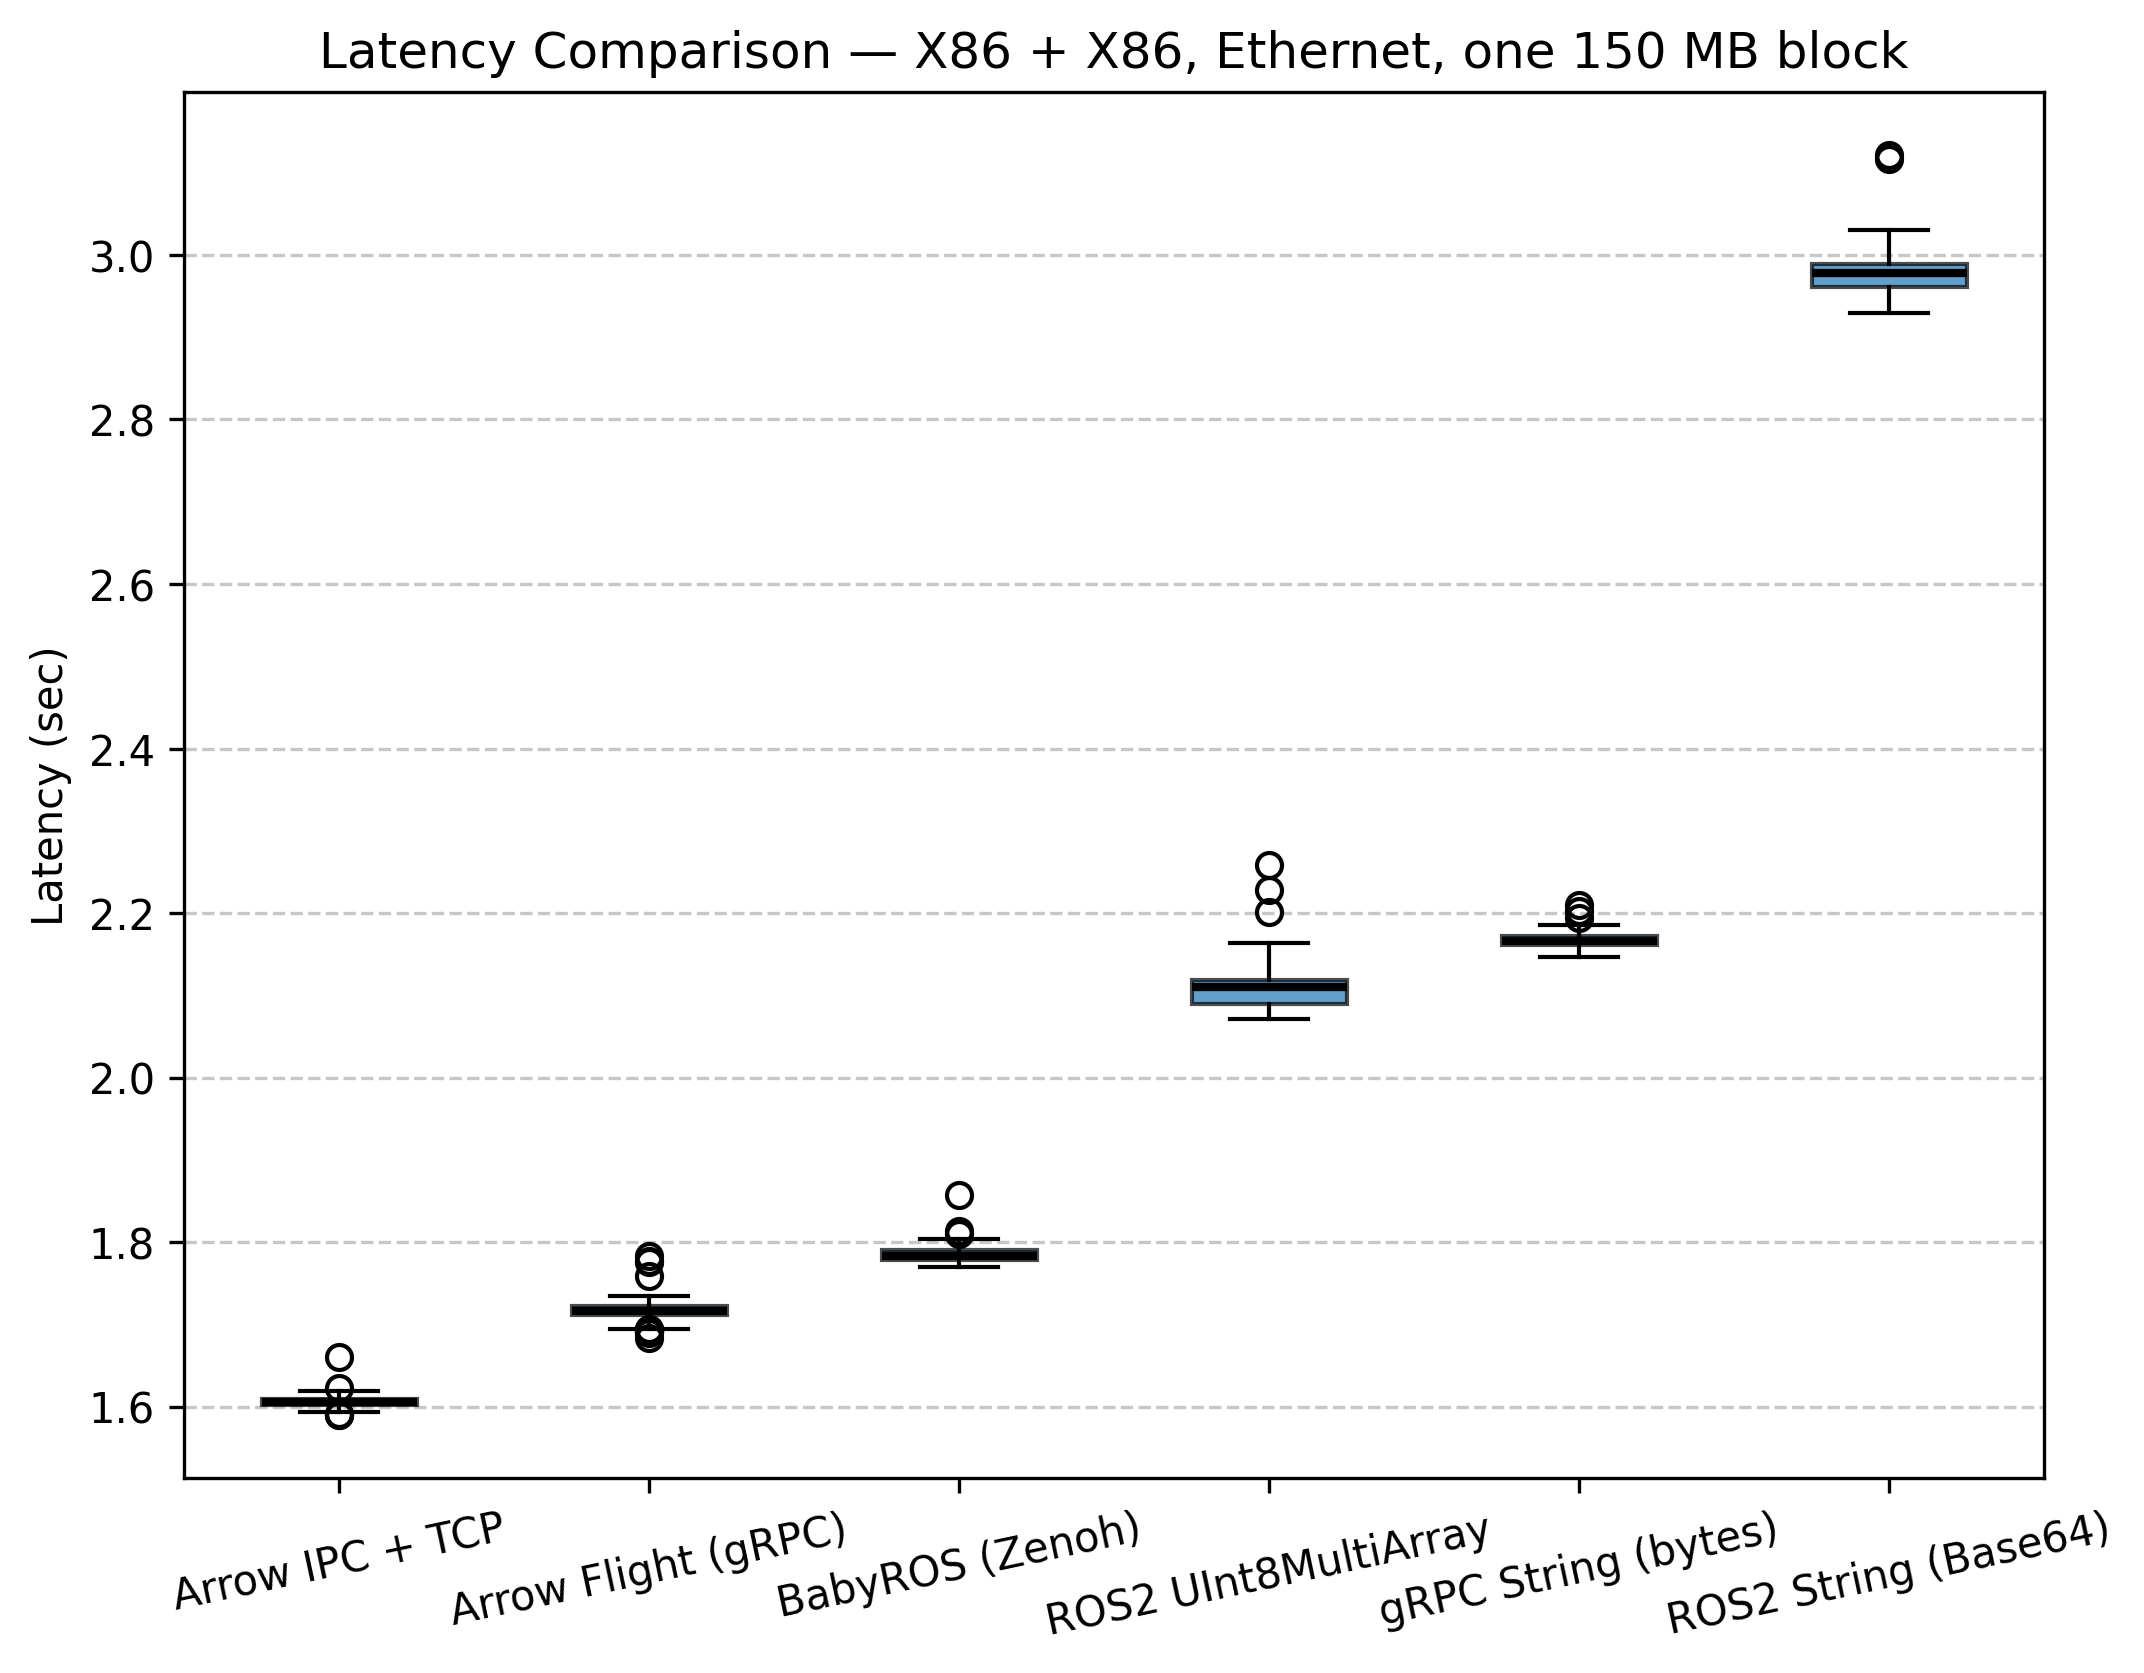
\includegraphics[width=\linewidth]{analysis/ethernet/plots_all/x86_machines/latency_boxplot.png}
    \caption{x86 receiver}
  \end{subfigure}\hfill
  \begin{subfigure}{0.49\linewidth}
    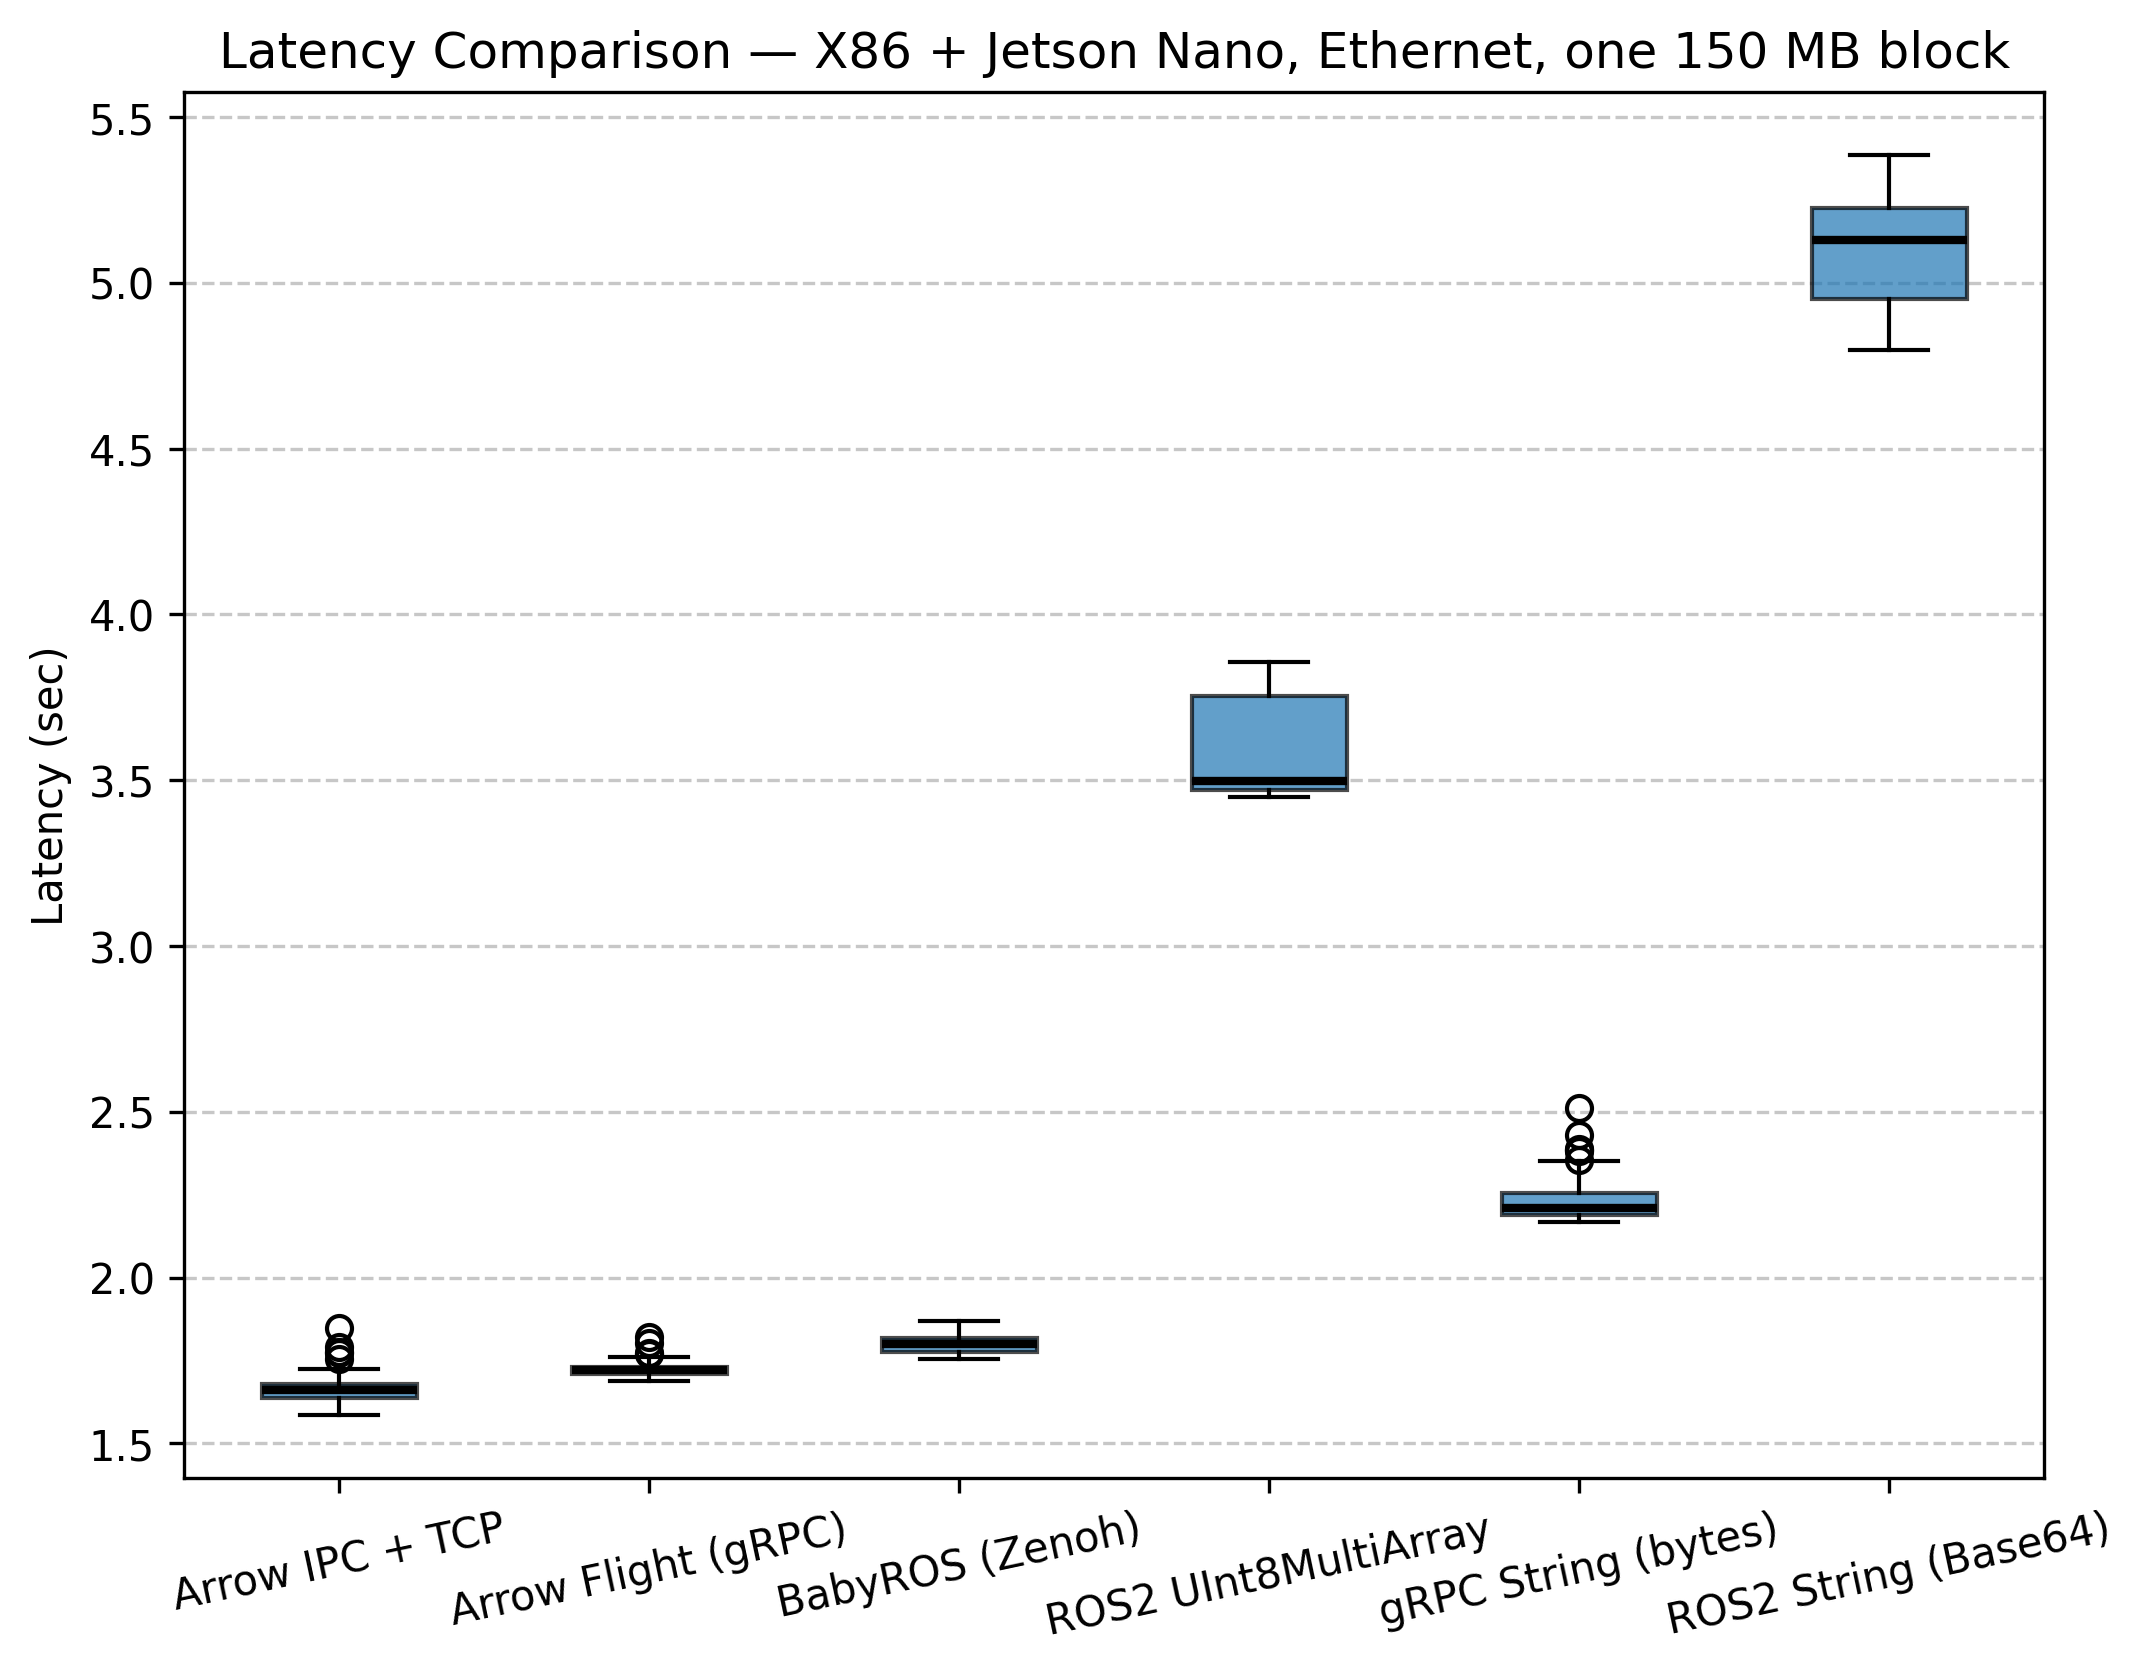
\includegraphics[width=\linewidth]{analysis/ethernet/plots_all/diff_machines/latency_boxplot.png}
    \caption{Jetson Nano receiver}
  \end{subfigure}
  \caption{Latency distributions of all methods for the single 150\,MB array.}
  \label{fig:single}
\end{figure}

\begin{figure}[t]
  \centering
  \begin{subfigure}{0.49\linewidth}
    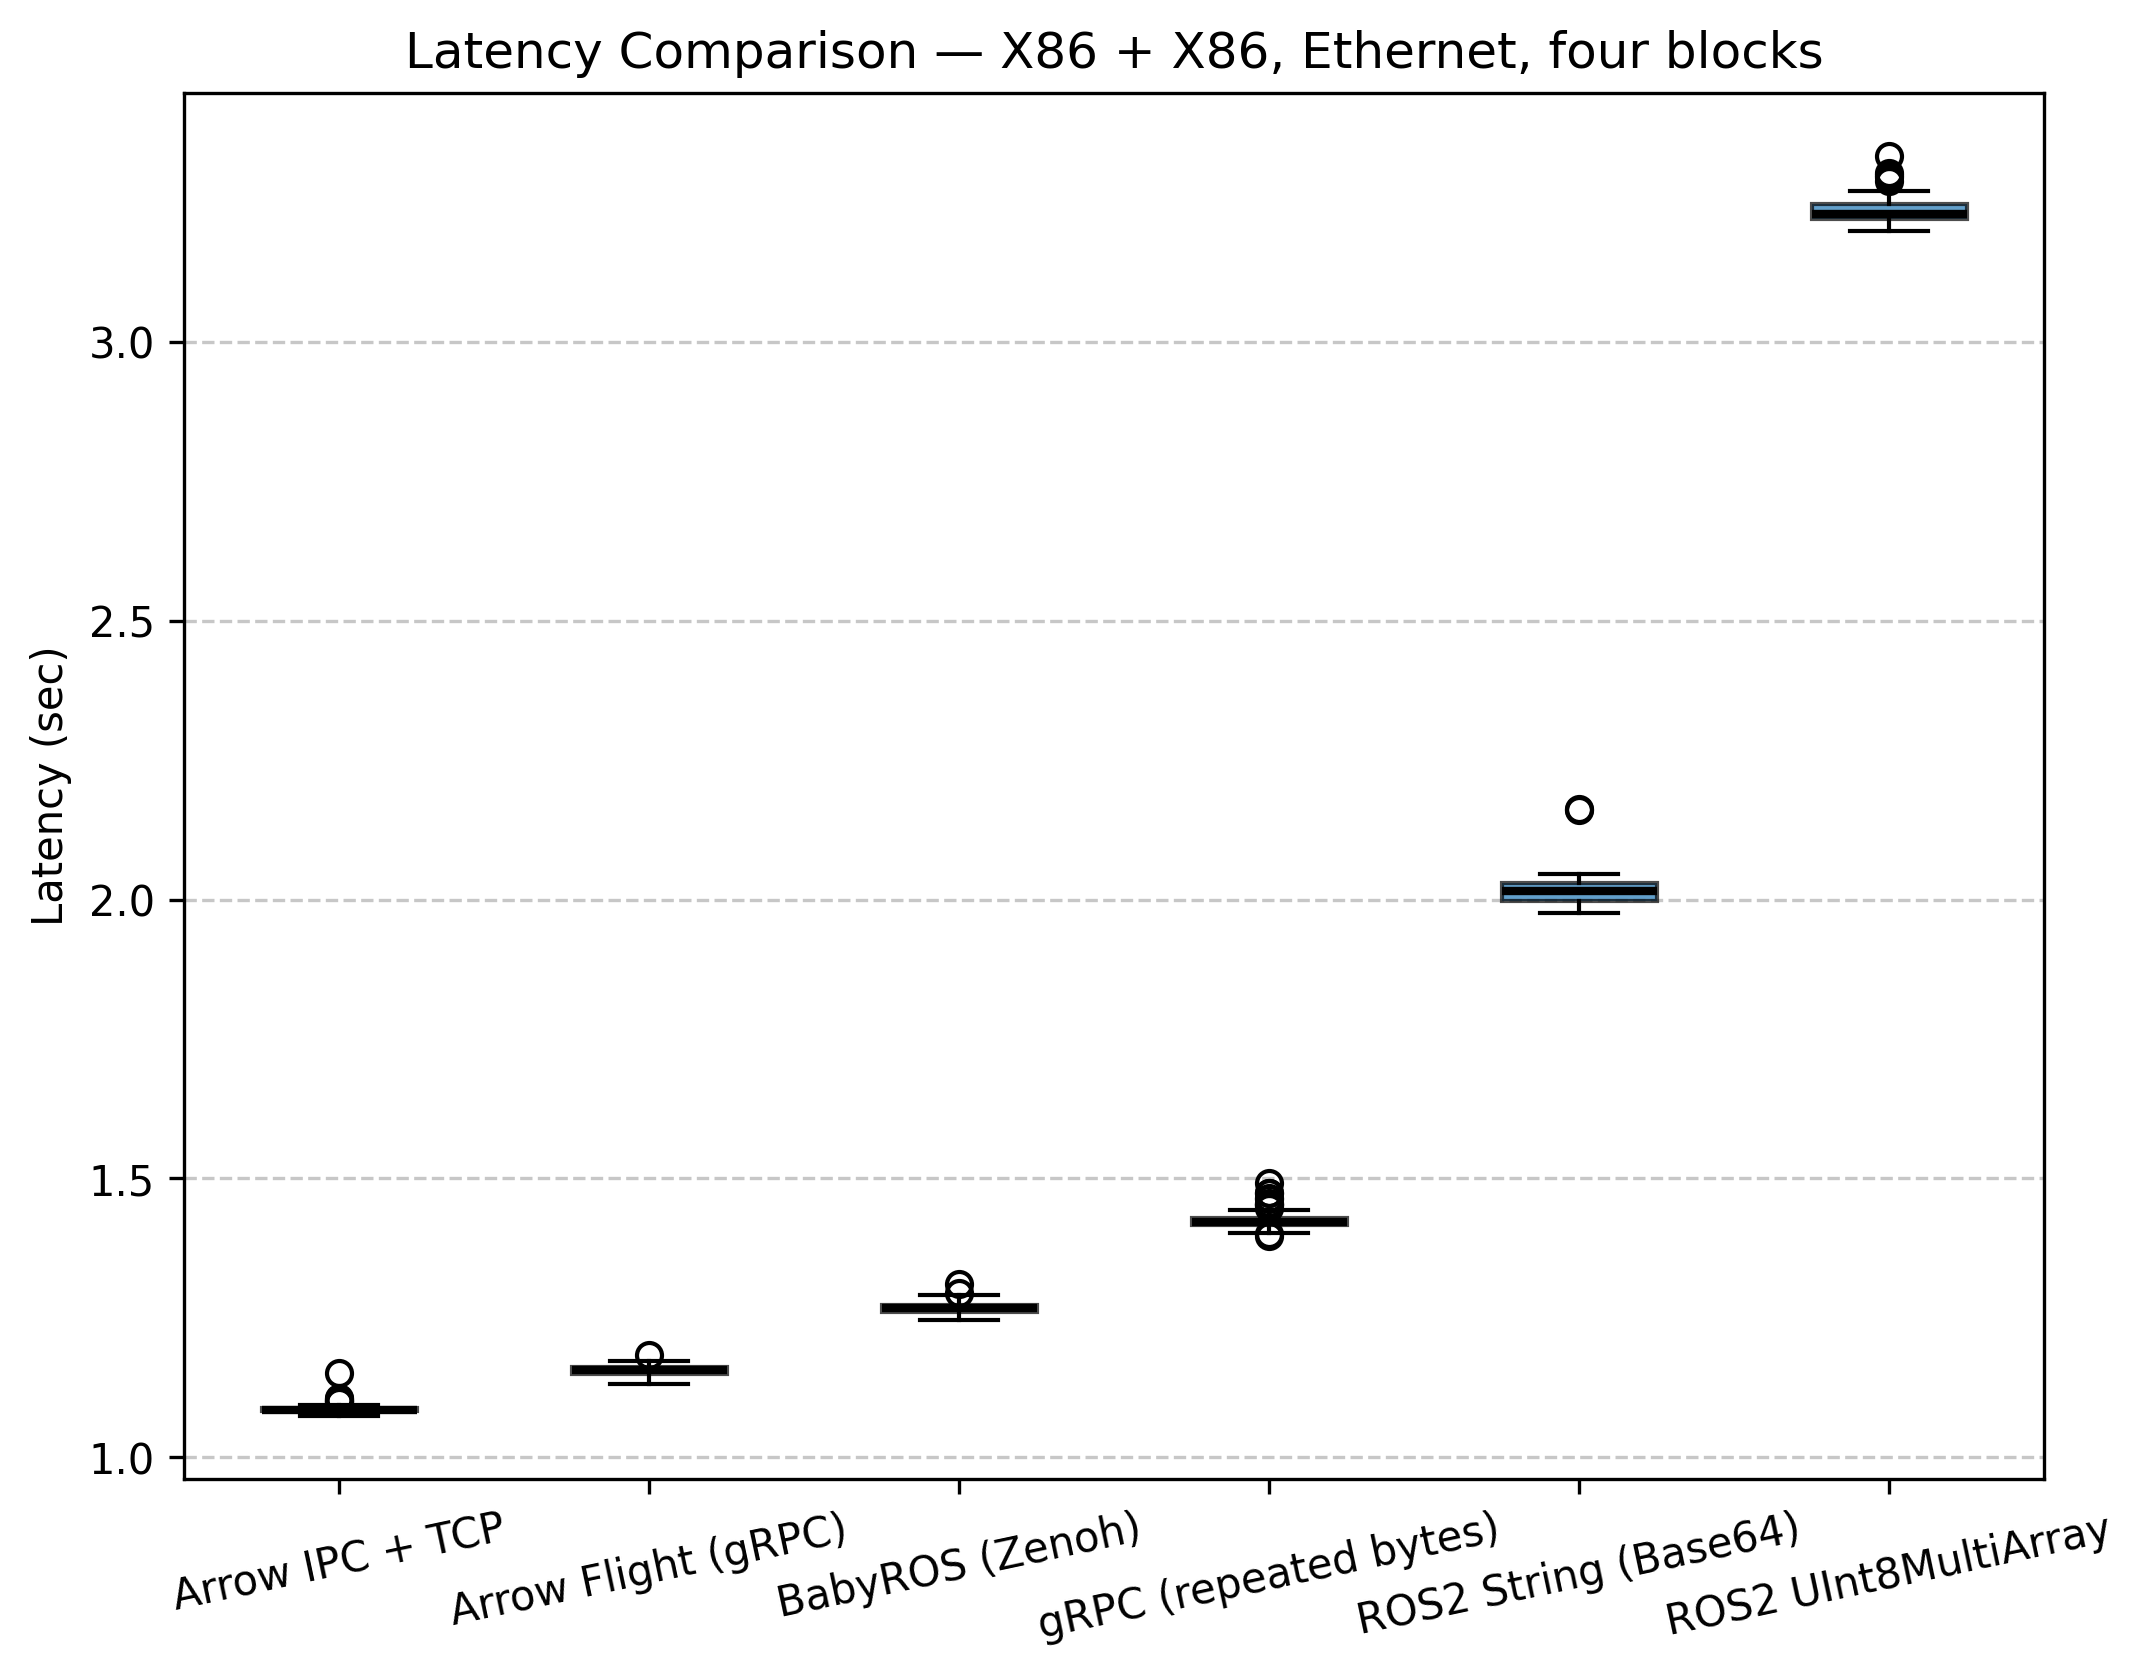
\includegraphics[width=\linewidth]{analysis/ethernet/plots_all_2nd/x86_machines/latency_boxplot.png}
    \caption{x86 receiver}
  \end{subfigure}\hfill
  \begin{subfigure}{0.49\linewidth}
    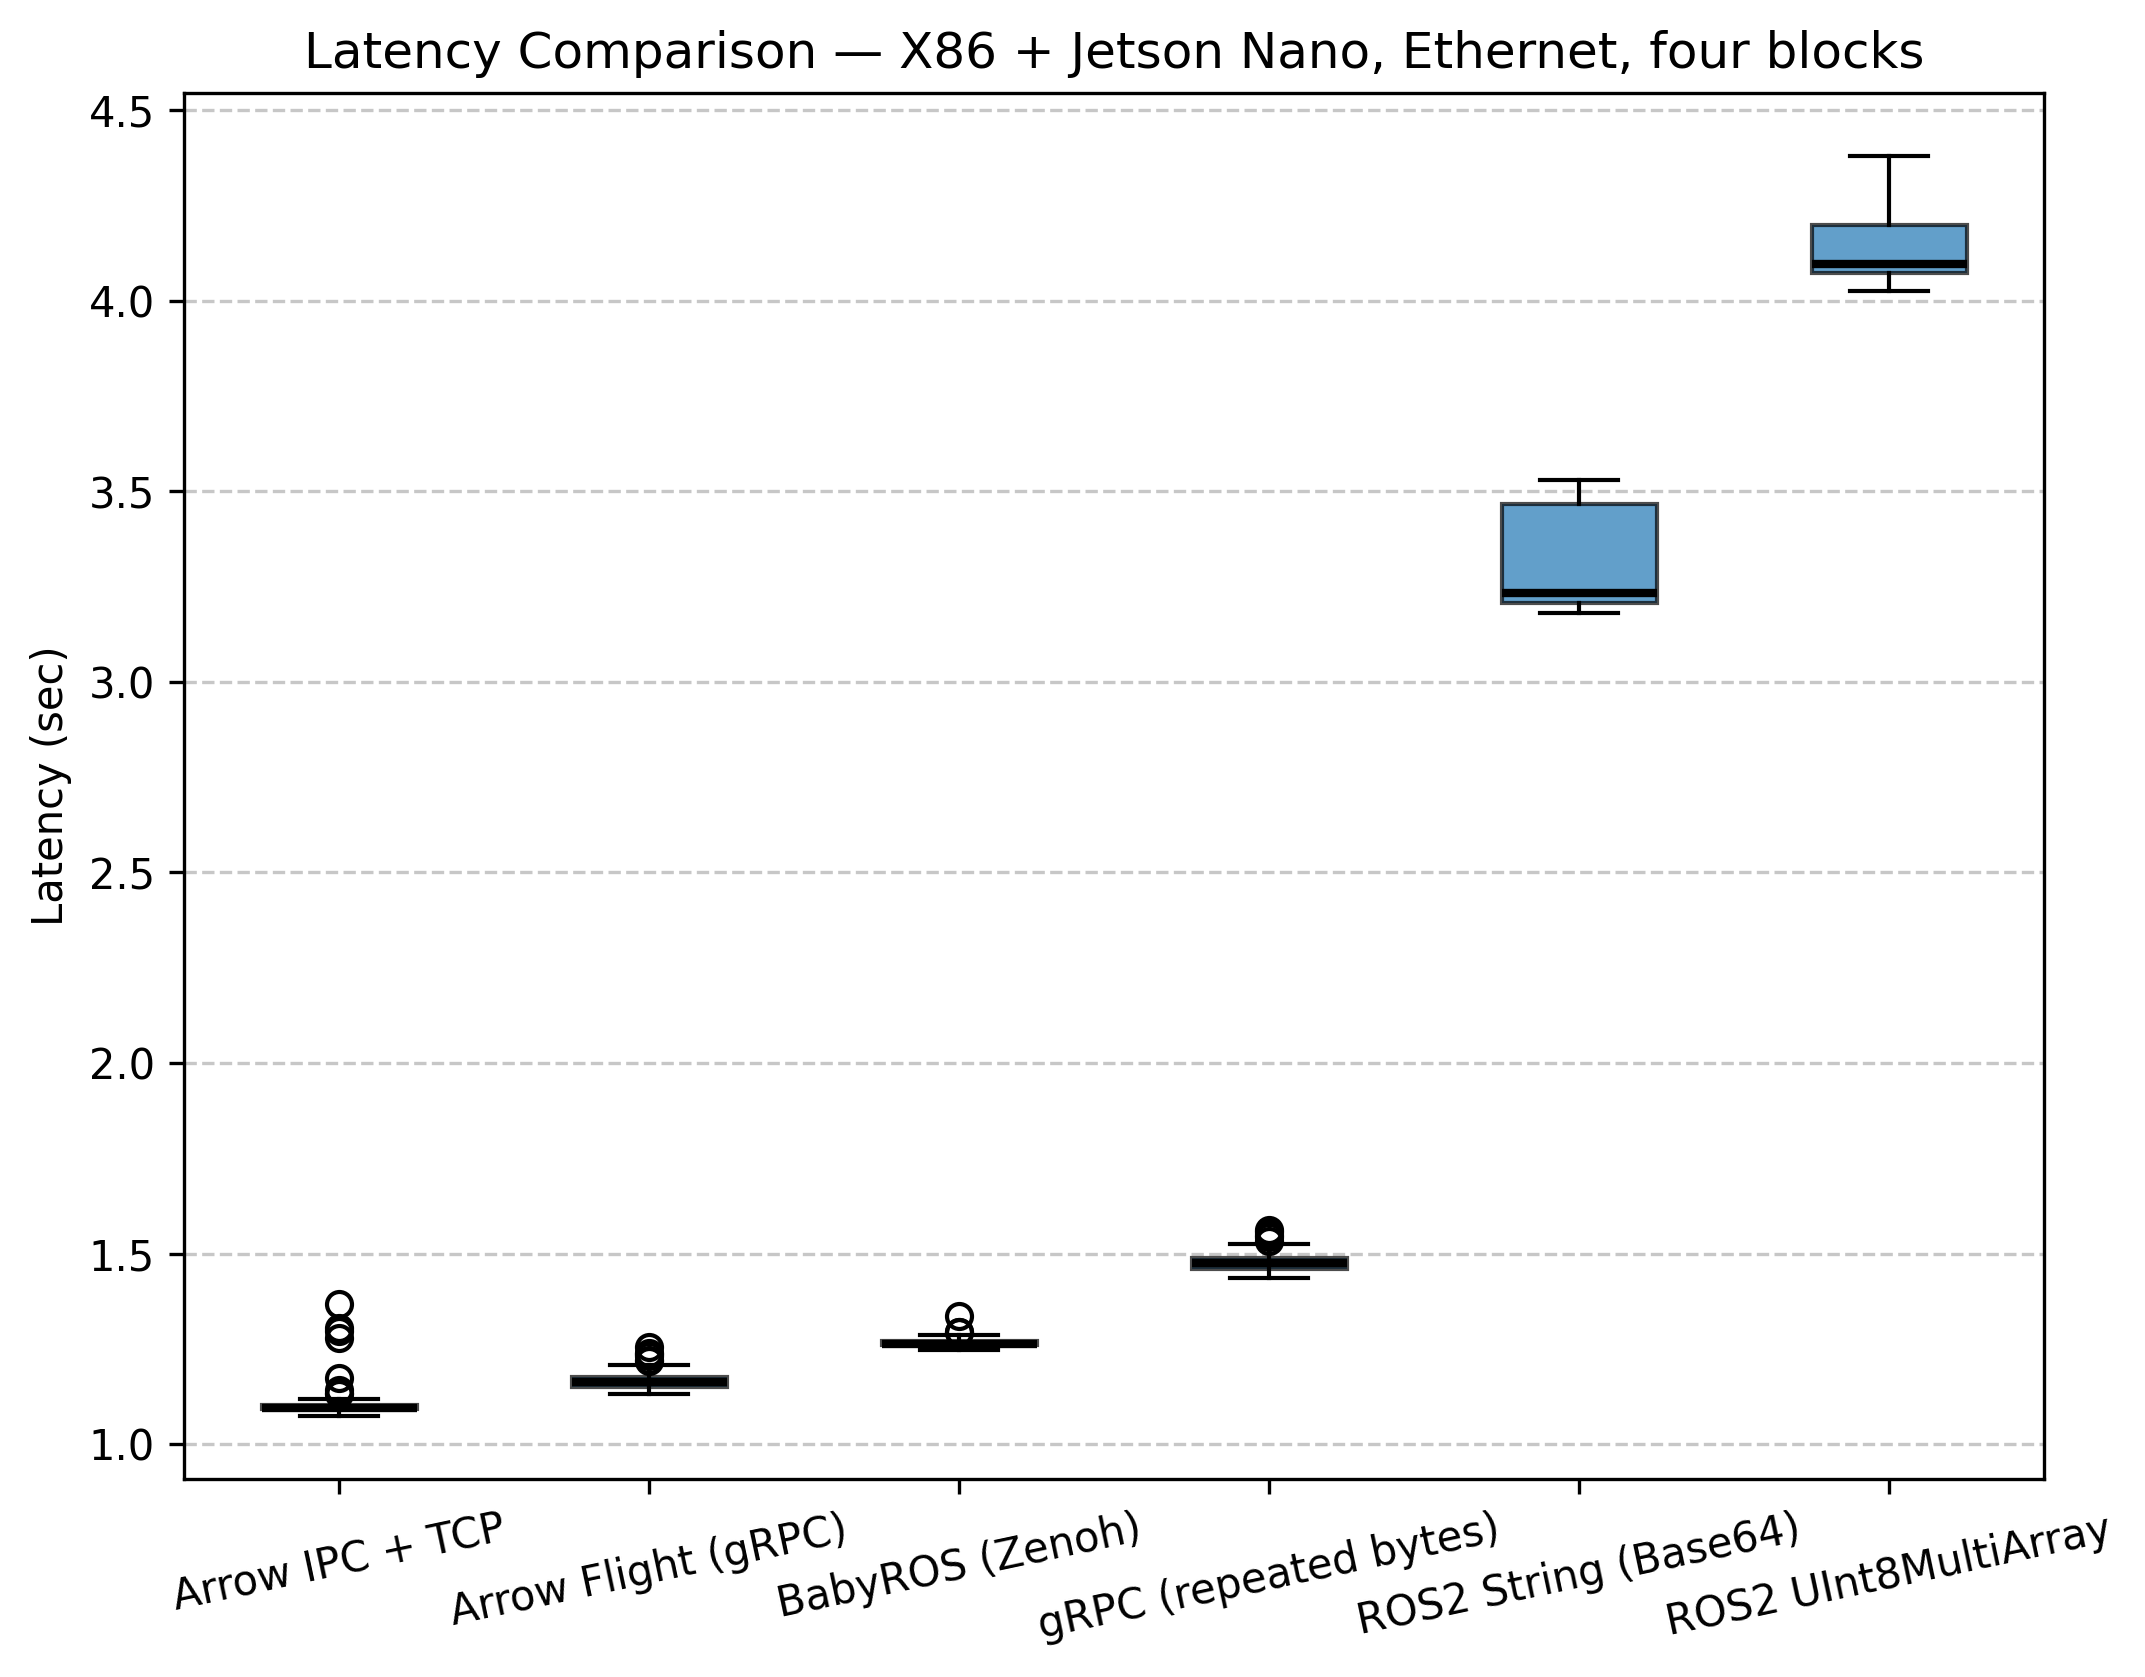
\includegraphics[width=\linewidth]{analysis/ethernet/plots_all_2nd/diff_machines/latency_boxplot.png}
    \caption{Jetson Nano receiver}
  \end{subfigure}
  \caption{Latency distributions of all methods for four arrays (98.8\,MB).}
  \label{fig:four}
\end{figure}

Three patterns emerge from this comparison.

First, the non-ROS technologies keep the same order in all four configurations. Arrow
IPC is always the fastest, reaching 76--79\,\% of the TCP goodput. It is followed by
Arrow Flight (3.5--6.9\,\% slower), BabyROS (8.0--16.7\,\% slower) and gRPC
(31--35\,\% slower).

Second, only ROS~2 is sensitive to the receiver hardware. Moving from the x86 receiver
to the Jetson Nano changes the latency of the non-ROS technologies by at most
3.7\,\%, whereas ROS~2 becomes 28--71\,\% slower. This penalty grows in proportion
to message size, at 9.3--10.5\,ms per MB for both message types and both payloads. As
a result, the best ROS~2 message type falls further behind Arrow IPC. It is
1.3--1.9$\times$ slower on the x86 receiver and 2.2--3.0$\times$ slower on the Jetson
Nano.

Third, which ROS~2 message type performs better depends on how the payload is packed.
\texttt{UInt8MultiArray} wins for the single array, which is assigned as
\texttt{bytes}. It loses for the four arrays, which pass through a Python list
conversion. That conversion costs more than Base64's 33\,\% size overhead.
